% ---------------------------------------------------------------------
\documentclass{article}

\usepackage{nberpreamble}
\title{\bfseries Notes on Simulating Power}
\author{\sffamily Prepared by Mauricio C\'aceres}
\date{\sffamily \today}

\usepackage{pgfplots}  % awesome plotting
\usepackage{tikz}      % vector graphics!
\usetikzlibrary{
  arrows,
  patterns,
  positioning,
  calc,
  fit,
  intersections,
  decorations.text,
  decorations.markings,
  decorations.pathmorphing,
  shadows.blur
}

\pgfplotsset{
  compat      = newest,
  axis x line = middle,
  axis y line = center,
  tick align  = outside,
  yticklabels = {,,},
  xticklabels = {,,},
  xtick       = {0},
  ytick       = {0}
}

\renewcommand{\displayoptions}{
  \maketitle
  \pagenumbering{arabic}
}

% ---------------------------------------------------------------------
\begin{document}
\displayoptions

%----------------------------------------------------------------------
\section{Parametric Power}
\label{sec:parametric_power}

We typically consider the model
\begin{equation}
Y_i = \alpha + \beta T_i + \gamma X_i + \varepsilon_i
\end{equation}

for some treatment $T_i$ at the individual level and the OLS estimator $\widehat{\beta}_{OLS}$ the difference in outcomes for the treatment and control groups. For $H_0: \beta = 0$, consider the rejection probability function
\begin{equation}
\pi_{N}(\beta) = P\set{\text{reject $H_0$} | \beta}
\end{equation}

For $\beta = 0$, this is $\alpha$ the probability of Type I error or \textit{significance}: How likely are we to make a mistake? For $\beta = \widetilde{\beta} \ne 0$ this is \textit{power}, the probability of rejecting the null: How likely are we to get it right? $\widehat{\beta}_{OLS}$ is $\sqrt{n}$-consistent, that is,
\[
  \sqrt{n} \left(\widehat{\beta}_{OLS} - \beta\right)
  \xrightarrow{D} N(0, V_{\widehat{\beta}})
\]

where $\beta$ is the true mean. Relying on large-sample asymptotics, we can visualize $\pi_N(\beta)$,
\begin{figure}[H]
  \centering
  \caption{Power of a Test}
  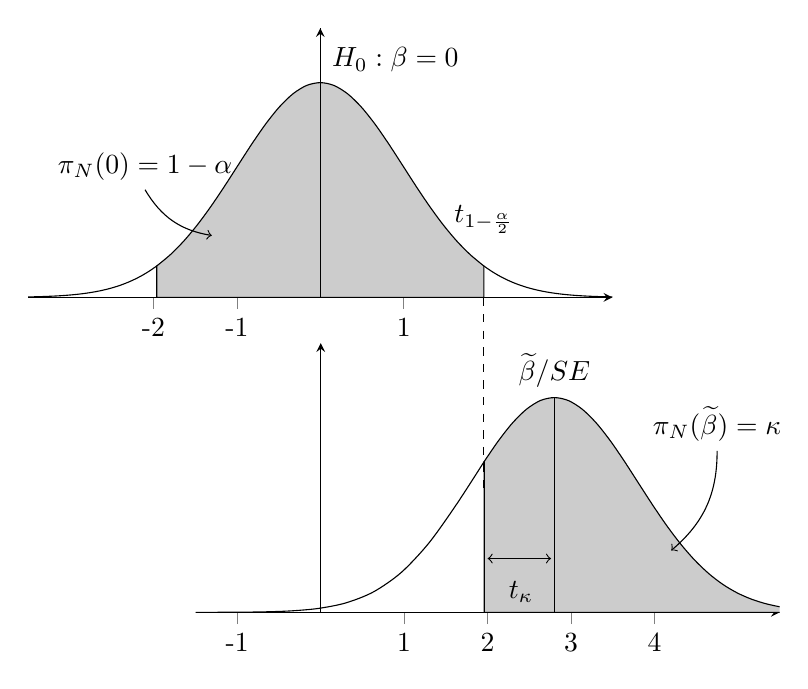
\begin{tikzpicture}
    \begin{axis}[name=plot1
      %,title=
      ,width=9cm
      ,height=5cm
      ,ymin=0
      ,ymax=0.5
      ,xmin=-1.5
      ,xmax=5.5
      ,domain=-6:6
      ,xticklabels = {-1,0,1,2,3,4}
      ,xtick = {-1,0,1,2,3,4}
      ]
      \addplot [fill=black!20,smooth,domain=1.96:6] {exp( - (x - 2.8)^2 / 2) / sqrt(2 * pi * 1)} \closedcycle;
      \addplot [smooth,domain=-6:1.96] {exp( - (x - 2.8)^2 / 2) / sqrt(2 * pi * 1)};
      \draw [-] (axis cs:2.8, 0) -- (axis cs:2.8, 0.399);
      \draw [<->] (axis cs:2, 0.1) -- (axis cs:2.76, 0.1);
      \node[above] at (axis cs:2.4, 0) {$t_{\kappa}$};
      \node[above] at (axis cs:2.8, 0.4) {$\widetilde{\beta} / SE$};
      \draw [->] (axis cs:4.75, 0.3) to[bend left=25] (axis cs:4.2, 0.115)
        node[above] at (axis cs:4.75, 0.3) {$\pi_N(\widetilde{\beta}) = \kappa$};
    \end{axis}
    \begin{axis}[name=plot2
      ,title={}
      ,at={($(plot1.south) + (-2.125cm, 4cm)$)}
      ,anchor=south
      ,width=9cm
      ,height=5cm
      ,ymin=0
      ,ymax=0.5
      ,xmin=-3.5
      ,xmax=3.5
      ,domain=-4:4
      ,xticklabels = {-2,-1,0,1}
      ,xtick = {-2,-1,0,1}
      ]
      \addplot [fill=black!20,smooth,domain=-1.96:1.96] {exp( - (x - 0)^2 / 2) / sqrt(2 * pi * 1)} \closedcycle;
      \addplot [smooth,domain=-4:-1.96] {exp( - (x - 0)^2 / 2) / sqrt(2 * pi * 1)};
      \addplot [smooth,domain=1.96:4] {exp( - (x - 0)^2 / 2) / sqrt(2 * pi * 1)};
      \draw [smooth] (axis cs:0, 0) -- (axis cs:0, 0.5);
      \node[above] at (axis cs:1.96, 0.1) {$t_{1 - \frac{\alpha}{2}}$};
      \node[above] at (axis cs:0.9, 0.4) {$H_0: \beta = 0$};
      \draw [->] (axis cs:-2.1, 0.2) to[bend right=25] (axis cs:-1.3, 0.115)
        node[above] at (axis cs:-2.1, 0.2) {$\pi_N(0) = 1 - \alpha$};
    \end{axis}
    \draw [dashed] (3.66, 4) -- (3.66, 1.5);
  \end{tikzpicture}
  \label{fig:power_of_a_test}
\end{figure}

A \textit{parametric} approach to power estimates $\widetilde{\beta}$ given $\alpha, \kappa, N, SE$ and terms it the \textit{minimum detectable effect}, MDE, or it estimates $N$ given $\alpha, \kappa, SE, MDE$.

%----------------------------------------------------------------------
\section{Simulated Confidence Interval}
\label{sec:simulated_confidence_interval}

However, it is possible to follow a \textit{non-parametric} approach to estimating power. Note there are $C = \left(\begin{smallmatrix} N \\ NP \end{smallmatrix}\right)$ ways to treat $PN$ individuals. If we estimate $\widehat{\beta}_{OLS}$ for each $c = 1, \ldots, C$, then we would know the exact distribution of our estimator for the treatment effect under the null given the data. Thus we could compute an exact $p$-value and determine whether to reject the null.

Even for modestly-sized data, $C$ will be intractably large. Hence we simulate $K$ draws from the possible treatment-control arrangements, $T_{ik}$ such that $\sum^{N}_{i = 1} T_{ik} = PN$, and estimate
\begin{equation}
Y_i = \alpha + \beta_k T_{ik} + \gamma X_i + \varepsilon_i
\label{eq:ri_ci_reg}
\end{equation}

Here $\widehat{\beta}_k$ will be distributed around $0$ and a $1 - \alpha$ CI under the null is given by
\begin{equation}
\widehat{CI}_{1 - \alpha} = \left(\widehat{F}^{-1}(\alpha / 2), \widehat{F}^{-1}(1 - \alpha / 2)\right)
\label{eq:ri_ci_hat}
\end{equation}

with $\widehat{F}(\widehat{\beta}_k)$ the empirical cdf of $\widehat{\beta}_k$. This approach is appealing compared to a parametric approach because it naturally takes into account the correlation structure of the errors, whereas a parametric approach requires making an assumption about $V_{\widehat{\beta}}$. If we had historical data on our study population (we can think of historical data as data on a population where our treatment had no effect, or the counterfactual of what would happen were we to treat our population with no effect) then we can simulate the CI above, and say that we expect to be able to reject effects outside the confidence interval.

%----------------------------------------------------------------------
\section{Simulated Power}
\label{sec:simulated_power}

Note, however, that this says nothing about power. In fact, power at either end of the confidence interval should be about $0.5$ (if $\widehat{\beta}_{OLS}$ were to be symmetrically distributed). Typically we look for a power level of $0.8$ or $0.9$. We could assume that the true effect of $T_i$ is $\widetilde{\beta}$, and estimate
\begin{equation}
  \begin{array}{r@{\hskip 4.5pt}l}
    \widetilde{Y}_{ik} & = Y_{i} + \widetilde{\beta} T_{ik} \\
    \widetilde{Y}_{ik} & = \alpha + \beta_k T_{ik} + \gamma X_{i} + \varepsilon_{i}
  \end{array}
\label{eq:ri_power_reg}
\end{equation}

In this case, $\widehat{\beta}_k$ will be distributed around $\widetilde{\beta}$ but the shape of the distribution would not have changed. Thus we can estimate power as
\begin{equation}
\widehat{\kappa} = \dfrac{1}{K} \sum^{}_{k} 1\left(\widehat{\beta}_k \notin \widehat{CI}_{1 - \alpha}\right)
\label{eq:ri_power_hat}
\end{equation}

and we we can search for $\widetilde{\beta}$ such that $\widehat{\kappa} \approx \kappa$ for some desired power level $\kappa$ (note $\widehat{\kappa} \xrightarrow{P} P\left(\beta_k \notin CI_{1 - \alpha}\right) = \kappa$). That is, we look for a $\widetilde{\beta}$ that causes us to reject the null $\kappa$ portion of the time. This is more complicated if $Y_i$ is binary. The approach works to obtain a CI under the null but the subsequent search does not map trivially. One idea is to randomly swap successes to failures (or the converse) based on $\widetilde{\beta}$. Consider
\begin{equation}
  \begin{array}{r@{\hskip 4.5pt}l}
    \widetilde{Y}_{ik} & = Y_{i} (1 - T_{ik}) + (Y_i + S_{ik}) T_{ik}  = Y_i + S_{ik} T_{ik} \\
    \widetilde{Y}_{ik} & = \alpha + \beta_k T_{ik} + \gamma X_{i} + \varepsilon_{i}
  \end{array}
\label{eq:ri_power_reg_binary}
\end{equation}

where $S_{ik}$ is constructed as follows
\begin{itemize}
  \item Let
    \begin{align*}
    T_k & = \sum^{}_{i} T_{ik}
    \quad\quad
    S_k = \sum^{}_{i} T_{ik} Y_i
    \\
    \widetilde{\beta} & \in \left[-\dfrac{S_k}{T_k}, \dfrac{T_k - S_k}{T_k}\right] \\
    S^1_k & = \widetilde{\beta} T_k \\
    S^2_k & =
      \begin{cases}
      \dfrac{S_k}{T_k} - S_{1k} & \widetilde{\beta} > 0  \\[9pt]
        \dfrac{T_k - S_k}{T_k} - S_{1k} & \widetilde{\beta} < 0
    \end{cases} \\
    \end{align*}

  \item Construct the set $\varsigma_k$ with $S^1_k$ entries equal to $1(\widetilde{\beta} > 0) - 1(\widetilde{\beta} < 0)$ and $S^2_k$ entries equal to $0$.

  \item For $i$ such that $T_{ik} = 1$, draw $s$ from $\varsigma_k$ \textit{without} replacement and set $S_{ik} = s$ ($S_{ik} = 0$ otherwise).
\end{itemize}

Note that $T^{-1}_k \sum^{}_{i} S_{ik} T_{ik} = \widetilde{\beta}$, hence
\begin{align*}
E\widehat{\beta}_k & = E\left[\widetilde{Y}_{ik} | T_{ik} = 1\right] - E\left[\widetilde{Y}_{ik} | T_{ik} = 0\right] \\
& = E\left[Y_i + S_{ik} | T_{ik} = 1\right] - E\left[Y_i | T_{ik} = 0\right] \\
& = EY_i + E\left[S_{ik} | T_{ik} = 1\right] - EY_i \\
& = \widetilde{\beta}
\end{align*}

So $\widehat{\beta}_k$ will be distributed around $\widetilde{\beta}$. Now we can outline a general simulation procedure:
\begin{enumerate}
\item Estimate a $1 - \alpha$ CI for $\widehat{\beta}_{OLS}$ under $H_0: \beta = 0$ using \Cref{eq:ri_ci_reg} and \Cref{eq:ri_ci_hat}.

\item Choose a starting MDE, $\widetilde{\beta}$, and estimate $\widehat{\beta}_k$ for $k = 1, \ldots, K$ using \Cref{eq:ri_power_reg} if $Y_i$ is continuous or \Cref{eq:ri_power_reg_binary} if $Y_i$ is binary.

\item Estimate power using \Cref{eq:ri_power_hat}.

\item If $\widehat{\kappa} < \kappa$ then increase $\widetilde{\beta}$; if $\widehat{\kappa} > \kappa$ then decrease $\widetilde{\beta}$.

\item Continue until $\left|\widehat{\kappa} - \kappa\right| < \epsilon$ for $\epsilon$ small.
\end{enumerate}

%----------------------------------------------------------------------
\section{Monte Carlo Simulations}
\label{sec:monte_carlo_simulations}

Consider some data-generating process (DGP) for $w_i = (y_i, x_i, T_i)$,
\[
  x_i \sim F_x
  \quad\quad
  T_i \sim \text{Bernoulli}(P)
  \quad\quad
  T_i \indep x_i
  \quad\quad
  y_i | x_i, T_i \sim F_y
\]

where
\[
\beta = E(y_i | T_i = 1, x_i) - E(y_i | T_i = 0, x_i)
\]

The aim is to compute the power of testing $\widehat{\beta}_{OLS}$ against our simulated confidence interval. For $m = 1, \ldots, M$:
\begin{enumerate}
\item Generate two draws from the DGP, $w_{1m}$ with $P = 0$ and $w_{2m}$ $P \in (0, 1)$.

\item Compute $\widehat{\kappa}_{1m}, \widehat{\kappa}_{2m}$ from our power simulation procedure and $\widehat{\beta}_{1m}, \widehat{\beta}_{2m}$ from OLS.

\item Construct a $1 - \alpha$ confidence interval for $\beta$, $\widehat{CI}^M_{1 - \alpha}$, using \Cref{eq:ri_ci_hat} and compute
\[
  \overline{\kappa}^M = \dfrac{1}{M} \sum^{}_{m} 1\left(
      \widehat{\beta}_{2m} \notin \widehat{CI}^M_{1 - \alpha}
  \right)
\]

\item It should be the case that $\widehat{\kappa}_{1m}$ are distributed around $\alpha$ and $\widehat{\kappa}_{2m}$ are distributed around $\overline{\kappa}^M$.
\end{enumerate}

% We use the procedure above to see if we can empirically match what power should be under known conditions. Consider the standard formula for MDE
% \begin{equation}
% MDE = (z_{\alpha / 2} + z_{\kappa}) \sqrt{\dfrac{\sigma_\varepsilon^2}{P (1 - P) N}}
% \end{equation}
%
% We can recover power as
% \begin{equation}
% \kappa = \Phi\left(MDE \sqrt{\dfrac{P (1 - P) N}{\sigma^2_\varepsilon}} - t_{\alpha / 2}\right)
% \end{equation}


% TODO: Finish writing this out. // 2016-09-02 14:33 EDT
% TODO: Actually code this up // 2016-09-02 14:33 EDT

% ---------------------------------------------------------------------
\end{document}
